\chapter{CUDA: A General Purpose Parallel Computing Architecture}
The first ever commercial graphics processing unit (GPU) was designed by NVIDIA in 1999. Because of the ever increasing demand for producing real-time graphics, which requires high arithmetic throughput, manufacturers have always focused on increasing the parallel processing capabilities of the GPUs. Today, GPUs outperform CPUs both in arithmetic processing efficiency and memory bandwidth \cite{nickolls,glaskowsky}.

Since 2003, efforts have been made to use GPUs even for non-graphics applications, especially for scientific work so that their high arithmetic throughput can be fully exploited. In our work we have used NVIDIA's Tesla C1060 and Fermi-based Tesla C2070 GPU cards. For implementing K-means algorithm on GPU, we have used Compute Unified Device Architecture (CUDA) \cite{cuda} API. This chapter will provide a brief introduction to NVIDIA's GPU architecture and CUDA API. More detailed information is available in literature published by NVIDIA \cite{cudadocs,fermiWhitepaper} and in books written by Farber \cite{farber} and Kirk \cite{kirk}.

\section{GPU Architecture}
\subsection{Overview}
Tesla C2070 is based on NVIDIA's Fermi architecture. It contains 448 CUDA cores. These cores are organized in 14 Streaming Multiprocessors (SMs) each containing 32 cores or Streaming Processors(SP). Figure \ref{fig:fermi:arch} shows block diagram of Fermi GF100 GPU containing 16 SMs, two more than C2070 GPU card that we have used for our work. Figure \ref{fig:fermi:arch} also shows six 64-bit DRAM memory partitions that provide a 384-bit memory interface. C2070 can support 6GB of GDDR5 DRAM memory. For data transfer between CPU and GPU there is a host interface connecting GPU with CPU via PCI-Express.

\begin{figure}[h]
	\centerline{
   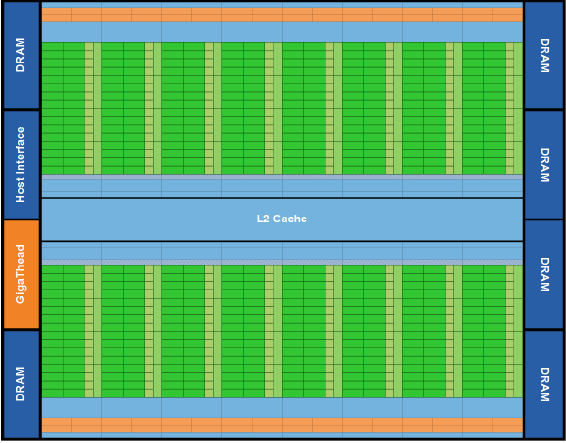
\includegraphics[width=0.8\textwidth]{./Data/nvidia/architecture_fermi}  	
	}
	\caption{ Block Diagram of G100 Fermi GPU containing 16 Streaming Multiprocessors (SMs) (Source: NVIDIA \cite{fermiWhitepaper}).}
\label{fig:fermi:arch}
\end{figure}

Fermi uses a {\it GigaThread} global scheduler to distribute execution blocks between the SMs. Each SM contains unified graphics and computing multiprocessors which execute vertex/geometry shader programs as well as parallel computing programs. We will be concentrating only on the parallel computing capabilities of SMs. A typical Fermi SM is shown in figure \ref{fig:fermi:sm}. Each SM contains 32 SIMT (Single-Instruction, Multiple-Thread) cores. 

\begin{figure}[h]
	\centerline{
   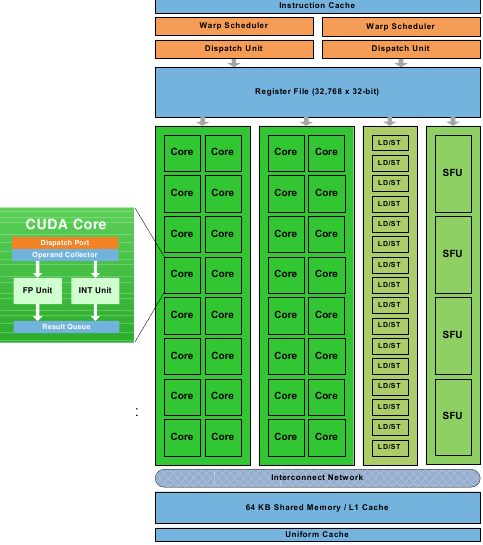
\includegraphics[width=0.8\textwidth]{./Data/nvidia/sm_fermi}  	
	}
	\caption{ Block Diagram of Fermi Streaming Multiprocessor (SM) containing 32 cores (Source: NVIDIA \cite{fermiWhitepaper}).}
\label{fig:fermi:sm}
\end{figure}

Each core contains a fully pipelined integer arithmetic logic unit (ALU) and floating point unit (FPU). Also, there are sixteen load/store units (LD/ST) to calculate source and destination addresses for sixteen threads per clock. Each SM contains four Special Function Units (SFUs) which execute transcendental instructions like sine, cosine and square root. Apart from register file, used for storing private variables, each SM also contains on-chip memory that is used for caching and sharing data between the cores. The instructions are fetched from instruction cache and are dispatched to the cores by two warp schedulers. More details about the on-chip memory and the warp schedulers is provided in the later sections.

\subsection{Memory Hierarchy}

Data reuse is an essential requirement for GPUs. This is due to the high latency of DRAM memory. To overcome this challenge caches have been provided, both inside SMs and also between the SMs and global memory, to cache regularly accessed data. Figure \ref{fig:fermi:mem} shows various memory partitions present in Fermi.

\begin{figure}[h]
	\centerline{
   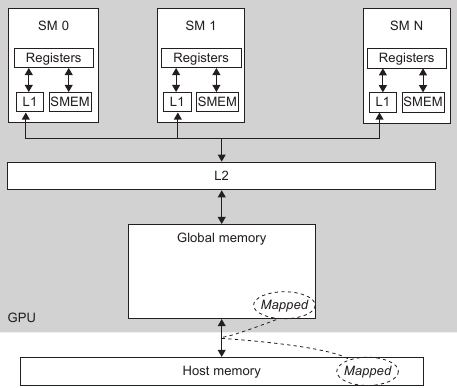
\includegraphics[width=0.8\textwidth]{./Data/nvidia/mem_fermi}  	
	}
	\caption{ CUDA memory hierarchy. (Source: NVIDIA \cite{farber}).}
\label{fig:fermi:mem}
\end{figure}

The global memory is stored in an external DRAM. It is used for communication between the SMs. Also any data transferred between CPU and GPU is also stored here. It is essential to coalesce global memory accesses to ensure single wide memory transactions. All the data accesses (both reads and writes) get cached in the unified L2 cache in an LRU fashion. It is 768 KB in size and helps in speeding up irregular accesses from global memory. Also it is coherent, ensuring all the cores receive updated values.

To further optimize data access from global memory a separate on-chip L1 cache is also present on each SM. It only caches memory reads and any stores directly go to L2 cache. It has been provided for exploiting spatial locality and uses 128  byte wide transactions. To make the L1 cache more configurable, it can be divided into L1 cache (maintained by SM) and shared memory (programmable). Shared memory can occupy either 16 KB or 48 KB from the 64 KB L1 cache. By storing data inside shared memory, the programmer can ensure that data which has to be reused over a long period of time stays inside the on-chip cache. L1 cache is shared between all the executing cores but unlike L2, it is not coherent and requires careful measures to ensure coherence.

Each executing core maintains its private data inside 32 K 32-bit registers. During execution the registers get partitioned among the cores statically and this partitioning can not be reconfigured till the execution finishes. As a result, if the private data cannot fit inside the available registers, it is spilled into the local memory. Fermi tries to accommodate the spilled data inside L1 cache which may lead to eviction of cached data.

Constant memory and texture memory are two other memory types present in Fermi. They both get cached on-chip and were of high importance in earlier models of NVIDIA GPUs because of unavailability of L2 and L1 caches. Constant memory is 64 KB in size and is read-only. In fact, one can get the same performance as from constant memory by declaring the data as constant inside global memory. Still, constant memory might become important if L2 cache is unable to accommodate all the data. But constant memory has a strong limitation. It only allows access of a single memory location at one time. Texture memory used to give better performance in comparison to global memory for non-coalesced data access on older GPUs. But with availability of L2 and L1 cache on Fermi, its advantage over global memory is very limited. It is more useful for visualization and shader programming.

\subsection{Hardware Multithreading}
A thread is the smallest execution unit on a GPU. Threads are created, managed, scheduled and executed by SM's SIMT multithreaded instruction unit in groups of 32 parallel threads called warps. Fermi SMs contain two warp schedulers which independently schedule alternate warps (see Figure \ref{fig:fermi:warp}). While one warp scheduler handles all the even warps, the other handles all the odd warps.
\begin{figure}[h]
	\centerline{
   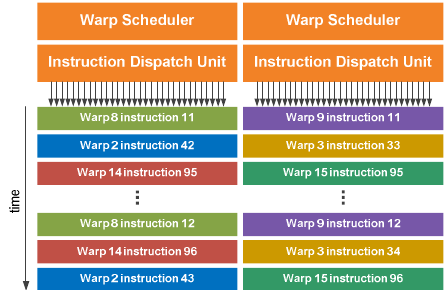
\includegraphics[width=0.8\textwidth]{./Data/nvidia/warp_fermi}  	
	}
	\caption{ Single-Instruction, Multiple-Thread (SIMT) warp execution on Fermi.(Source: NVIDIA \cite{fermiWhitepaper}).}
\label{fig:fermi:warp}
\end{figure}


A SIMT warp is composed of individual threads of the same type. All the threads start together at the same program address. Whenever the cores assigned to a warp scheduler are ready, the scheduler selects a warp that is ready to execute and issues the next instruction on that warp's active threads. The instruction gets broadcast to all the participant threads.

Due to branching and predication, a thread may be inactive and may not execute. Whenever threads diverge, all the branches are executed serially. All the threads that do not fall on a particular path are disabled. Once all the paths have been completed the participant threads again re-converge and start executing the next instruction simultaneously.

Serial execution due to branch divergence only happens inside a warp. Different warps can independently execute common or disjoint paths without effecting each other. Since each warp scheduler has 16 cores to execute upon, an issued warp instruction executes as two sets of 16 threads (half-warps) over two processor cycles. Also, the maximum number of warps that can reside simultaneously on an SM gets decided by the availability of resources (registers and shared memory).

\section{CUDA API}
\subsection{CUDA Execution Model}
During execution of CUDA programs, the program is executed with the GPU acting as a co-processor of CPU. While executing a GPU program, the code starts execution on the CPU. To ask the CPU to execute a piece of code on the GPU, a special call called kernel invocation is used. It is an asynchronous call to the CUDA driver which loads the program on GPU and control immediately comes back to the CPU to execute the next instruction. 
\begin{figure}[h]
	\centerline{
   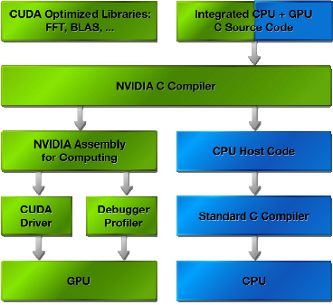
\includegraphics[width=0.6\textwidth]{./Data/nvidia/cuda_fermi}  	
	}
	\caption{ CUDA software stack.(Source: NVIDIA).}
\label{fig:fermi:cuda}
\end{figure}

All transfers of data, launching of GPU computing functions (kernels) and any other interaction between CPU and GPU are handled by the runtime driver. To map a large computational problem on the highly parallel GPU architecture, the problem is divided into smaller independent components that can be solved in parallel.

Before scheduling the large number of concurrent threads on to the GPU, they are partitioned into disjoint components called thread blocks. All threads in a thread block co-operate with each other and run on a single SM, executing the same set of instructions. Since the threads inside a block are present on the same SM, they can share the data among each other through shared memory and with constituent threads of other blocks through global memory.

While threads in a single warp always execute in a synchronized manner, the threads in a thread block can also synchronize using barrier synchronization functions. During kernel invocation, the total number of thread blocks and the number of threads present in each block need to be specified. On the basis of this information the resource usage (shared and register memory) of each block is calculated. The {\it GigaThread} scheduler then allocates maximum possible blocks to each SM.

After receiving the thread blocks, SM divides them into warps and allocates them to the warp schedulers. Finally, the two warp schedulers pick up one warp each which is ready to execute and start executing instructions. The remaining blocks which could not be allocated any SM wait for the current set of blocks to finish their execution. New thread blocks are only allocated to an SM after it has finished execution of all the thread blocks currently allotted to it.

\subsection{CUDA C Runtime}
For programming using CUDA, we have used CUDA's C Runtime API. We mention here few basic functions provided by the C runtime. An exhaustive listing is present in CUDA reference manual \cite{cuda}.
\begin{itemize}
\item {\bf Kernel invocation:} A kernel is declared like a normal C function except that it uses the qualifier, \_\_global\_\_.


\begin{lstlisting}
__global__ void firstKernel (void) {
}
\end{lstlisting}


While invoking a kernel we need to pass two parameters to it which specify the way thread blocks and threads inside individual thread blocks are going to be organized.

\begin{lstlisting}
firstKernel << grid_size, block_size >> ();
\end{lstlisting}

Here {\it grid\_size} specifies the grid size for blocks and {\it block\_size} specifies the grid size for threads inside every block.

\begin{lstlisting}
dim3 grid_size (gx, gy, gz);
dim3 block_size (bx, by, bz);
\end{lstlisting}

During kernel execution, each block and every thread inside it is assigned an index on the basis of their position in the grids we defined above.

\item {\bf Device functions:} Device functions use the qualifier \_\_device\_\_. A device function can only be invoked from code running on GPU.

\begin{lstlisting}
__device__ void firstDevice ( void ) {
}
__global__ void firstKernel ( void ) {
  firstDevice();
}
\end{lstlisting}

Also, Fermi GPUs allow device functions that are recursive in nature.


\item {\bf Memory allocation:} To allocate variables in device memory we use the function, {\it cudaMalloc}.

\begin{lstlisting}[morekeywords={cudaMalloc,cudaMemcpy,cudaMemcpyHostToDevice}]
// Allocate array in host memory
float *h_A = (float *)malloc(size);
// Allocate array in device memory
float *d_A;
cudaMalloc ( &d_A, size );
// Copy array from host memory to device memory
cudaMemcpy ( d_A, h_A, size, cudaMemcpyHostToDevice );
\end{lstlisting}

{\it cudaMemcpy} is used to copy data from host to device memory, or from device to device memory and from device to host memory.

\item {\bf CUDA events:} For performance benchmarking and runtime measurement, we have used events provided by CUDA.

\begin{lstlisting}[morekeywords={cudaEvent_t,cudaEventCreate,cudaEventRecord,cudaEventSynchronize,cudaEventElapsedTime,cudaEventDestroy}]
// Create the event variables.
cudaEvent_t start, stop;
cudaEventCreate(&start);
cudaEventCreate(&stop);

// Record the event when kernel starts.
cudaEventRecord(start, 0);
{
  firstKernel << grid_size,block_size >> ();
}
// Record the event when kernel stops.
cudaEventRecord(stop, 0);
// Wait for the asynchronous kernel to finish.
cudaEventSynchronize(stop);
// Store the elapsed time.
float elapsedTime;
cudaEventElapsedTime ( &elapsedTime, start, stop );

// Finally destroy the event variables.
cudaEventDestroy(start);
cudaEventDestroy(stop);
\end{lstlisting}
\end{itemize}

